\documentclass{ml}
\usepackage{graphicx}
\nameone{Franklin Hu}
\nametwo{Sunil Pedapudi}
\course{CS 194-10 Machine Learning}
\assignment{Assignment 7}

\begin{document}
\maketitle
\newcommand{\pr}{\mathbb{P}}

\begin{question}{Russell \& Norvig 14.7} % 1
    \part % a
        Diagram augmented with \(IcyWeather\) and \(StarterMotor\) \\
        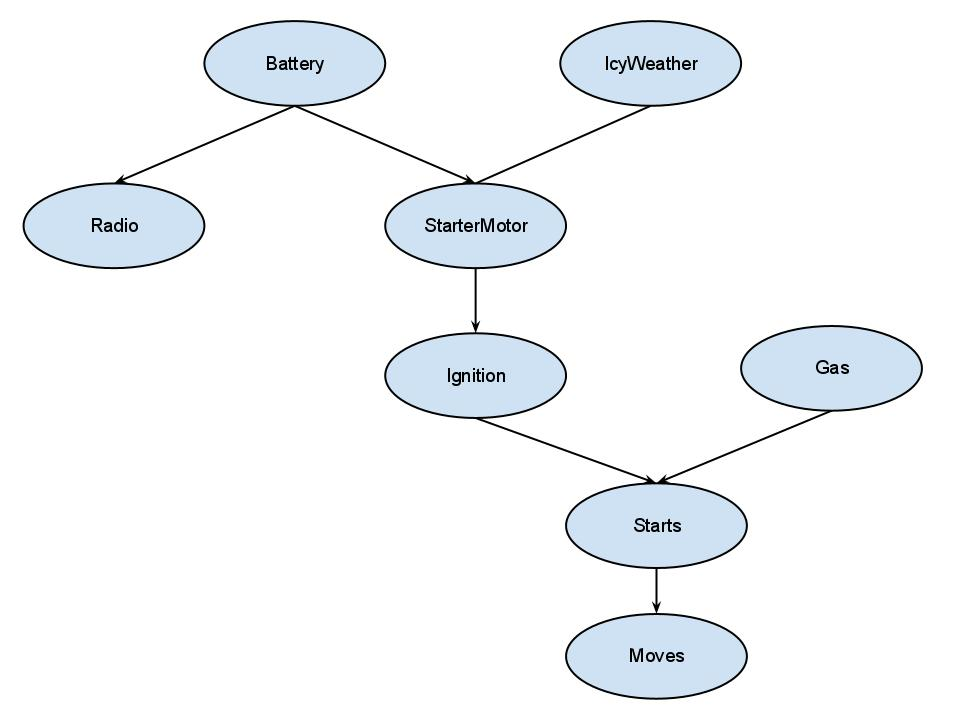
\includegraphics[scale=0.4]{1a.jpg}
    \part % b
        \begin{tabular}{l || c | c | c}
            x & P(Battery = x) & P(IcyWeather = x) & P(Gas = x)\\
            \hline
            true  & 0.8 & 0.4 & 0.9 \\
        \end{tabular}

        \begin{tabular}{l || c}
            b & P(Radio = true \(|\) Battery = b) \\
            \hline
            true & 0.9 \\
            false & 0.0 
        \end{tabular}

        \begin{tabular}{l | l || c}
            b & i & P(StarterMotor = true \(|\) Battery = b, IcyWeather = i) \\
            \hline
            true & true & 0.6 \\
            true & false & 0.9 \\
            false & true  & 0.01 \\
            false & false & 0.1
        \end{tabular}

        \begin{tabular}{l || c}
            s & P(Ignition = true \(|\) StarterMotor = s) \\
            \hline
            true & 0.99 \\
            false & 0.0
        \end{tabular}

        \begin{tabular}{l | l || c}
            i & g & P(Starts = true \(|\) Ignition = i, Gas = g) \\
            \hline
            true & true & 0.99 \\
            true & false & 0.0 \\
            false & true & 0.0 \\
            false & false & 0.0
        \end{tabular}

        \begin{tabular}{l || c}
            s & P(Moves = true \(|\) Starts = s) \\
            \hline
            true & 0.95
        \end{tabular}
    \part % c
        The joint probability distribution table for eight Boolean nodes
        would contain \(2^8=256\) independent values.
    \part % d
        The network tables for the diagram in (a) has: \\
        \begin{tabular}{c | c | c | c}
            NumParents & Node & Values per Node & Total \\
            \hline
            0 & 3 & 1 & 3 \\
            1 & 3 & 2 & 6 \\
            2 & 2 & 4 & 8
        \end{tabular} \\
        If we sum the right most column, we find that we have a total
        of \(17\) independent probability values in our Bayesian Network.
    \part % e
        The noisy-AND distribution can be thought of as a node in a
        Bayes Net that is true if some noisy combination of all its
        parents is also true. We can consider the \(Starts\) node
        as a noisy-AND since a car would require all of the parent 
        components to be functioning correctly for the car to start. \\
        The following equation may be a suitable noisy-AND distribution
        \begin{equation*}
            P(X=true|U_1,\hdots,U_D)=\prod\limits_{j=1}^D p_j
        \end{equation*}
        where \(U_1,\hdots,U_D\) are the parents of \(X\). By taking the
        product of the probabilities of the parents, the node \(X\)
        only has a high probability of being \(true\) if all the 
        parents also have a high probability.
\end{question} % 1

\begin{question}{Exponential Family} % 2 
    \part % a
    Given the form
    \begin{equation*}
      p(x) = h(x)exp{\theta^TT(x) - A(\theta)}
    \end{equation*}
    We can express
    \begin{enumerate}[(i)]
      \item
        \begin{align*}
          Normal(\mu,1)
          &= \frac{1}{\sqrt{2\pi}\sigma}e^{\frac{-(x-\mu)^2}{2\sigma^2}}\\
          &= \frac{1}{\sqrt{2\pi}}e^{\frac{-(x-\mu)^2}{2}}
        \end{align*}
        by choosing
        \begin{align*}
          h(x) &= \frac{e^{\frac{-x^2}{2}}}{\sqrt{2\pi}}\\
          T(x) &= x\\
          A(\theta) &= \frac{\mu^2}{2}\\
          \theta &= \mu
        \end{align*}
        which renders the form of a normal equation.

      \item
        \begin{equation*}
          Bernoulli(p) = p^x(1-p)^{1-x}
        \end{equation*}
        by choosing
        \begin{align*}
          h(x) &= p^k\\
          T(x) &= ln(1-p)\\
          \theta &= 1-x\\
          A(\theta) &= 0
        \end{align*}
        which recovers the original form of Bernoulli(\(p\))

      \item
        \begin{equation*}
          Categorical(p_1,\hdots,p_k) = \prod^n_{i=1}p_i^(x_i)
        \end{equation*}
        by choosing
        \begin{align*}
          h(x) &= 1\\
          \theta^T &= \textnormal{1-of-K encoded vector}\\
          T(x) &= \sum_{i=1}^Kp_i\\
          A(\theta) &= 0
        \end{align*}
    \end{enumerate}

    \part % b
    Let us first note that \(\pr(X = x,T(x) = t)\) is simply a function of \(x\)
    since \(T(x)\) is a function of \(x\). We assume that \(\theta\) is given in
    all scenarios.
    Then,
    \begin{align*}
      \pr(X = x, T(x) = t)
      &= \pr(X = x)\pr(T(x) = t)
    \end{align*}
    We then note that we can express
    \begin{align*}
      \pr(X = x, T(x) = t) &= f(x, t) = f(x)\\
      f(x, t) &= f(x)g(t)
    \end{align*}
    We intend to show the following.
    \begin{align*}
      f(t)
      &= \sum_{x s.t. T(x) = t} f(x,t)\\
      &= \sum_{x s.t. T(x) = t} f(x)\\
      &= \sum_{x s.t. T(x) = t} f(x)g(t)\\
      &= g(t)\sum_{x s.t. T(x) = t} f(x)
    \end{align*}
    Knowing this, we can find the conditional probability distribution
    \begin{align*}
      \pr(x|t)
      &= \frac{f(x,t)}{f(t)}\\
      &= \frac{f(x)}{f(t)}\\
      &= \frac{f(x)g(t)}{g(t)\sum_{x s.t. T(x) = t} f(x)}\\
      &= \frac{f(x)}{\sum_{x s.t. T(x) = t} f(x)}
    \end{align*}
    We observe that this function is dependent on x and not t, and can therefore
    conclude that the estimate is reliant on only \(T(x)\).
    \part % c
    From (a), we see that
    \begin{equation*}
      A(\theta) = \frac{\mu^2}{2}
    \end{equation*}
    Knowing
    \begin{align*}
      E[X = T(x)]
      &= E[X = x]\\
      &= \mu
    \end{align*}
    we show
    \begin{align*}
      \frac{\partial}{\partial\theta} A(\theta)
      &= \frac{\partial}{\partial\theta} A(\theta)\\
      \textnormal{Since \(\theta = \mu\)},\\
      &= \frac{\partial}{\partial\mu} A(\mu)\\
      &= \frac{\partial}{\partial\mu} \frac{\mu^2}{2}\\
      &= \mu &= E[T(x)]
    \end{align*}
\end{question} % 2

\begin{question}{EM with discrete variables} % 3
    \part % a
    \part % b
    \part % c
    
    Without loss of generality, no. The number of iterations can increase depending
    on the initial values chosen. In our situation, our initial values depended on
    pre-computation, but using random initial values can increase (or decrease) the
    total number of iterations until convergence. 
\end{question} % 3

\begin{question}{Learning with continuous variables} % 4
    \part % a
        Since \(P(Y_j|X=k)\sim N(\mu_{jk},\sigma^2)\), each element
        of the \(\textbf{Y}\) vector is independent so we can write
        the likelihood of the entire vector as a product of the
        likelihood of its elements. The log-likelihood similarly
        turns into a sum.
       \begin{align*}
            P(\textbf{Y}|X=k)
            &= \prod\limits_{j=1}^D P(Y_j|X=k) \\
            \log P(\textbf{Y}|X=k)
            &= \sum\limits_{j=1}^D \log P(Y_j|X=k)
        \end{align*}
        Given \(N\) i.i.d. observations of \((X,\textbf{Y},Z)\) that we
        call \(E_1, \hdots, E_N\), and \(\textbf{w}=\langle w_1, \hdots,
        w_D \rangle\):
        \begin{align*}
            P(E_1, \hdots, E_N)
            &= \prod\limits_{i=1}^N P(E_i) \\
            &= \prod\limits_{i=1}^N P(X_i=x_i,\textbf{Y}_i=\textbf{y}_i,
                Z_i=z_i) \\
            &= \prod\limits_{i=1}^N P(X_i=x_i) \cdot 
                P(\textbf{Y}_i=\textbf{y}_i|X_i=x_i) \cdot 
                P(Z_i=z_i|X_i=x_i,\textbf{Y}_i=\textbf{y}_i) \\
            &= \prod\limits_{i=1}^N P(X_i=x_i) \cdot 
                P(\textbf{Y}_i=y_i|X_i=x_i) \cdot 
                P(Z_i=z_i|\textbf{Y}_i=\textbf{y}_i) \\
            \log P(E_1, \hdots, E_N)
            &= \sum\limits_{i=1}^N \log P(X_i=x_i) + \log 
                P(\textbf{Y}_i=\textbf{y}_i|X_i=x_i) + \log 
                P(Z_i=z_i|\textbf{Y}_i=\textbf{y}_i) \\
            &= \sum\limits_{i=1}^N \log (0.5) + \left(
                \sum\limits_{j=1}^D \log P(Y_j=y_j|X_i=x_i) \right) + \log 
                P(Z_i=z|\textbf{Y}_i=\textbf{y}_i) \\
            &= \sum\limits_{i=1}^N -\log(2) + \left(
                \sum\limits_{j=1}^D \log \left( 
                \frac{1}{\sigma\sqrt{2\pi}} 
                \exp{\left(\frac{\mu_{j{x_i}}-y_j}{\sigma}\right)^2}
                \right) \right) +
                \log \left( \frac{1}{1+\exp \left(-z_i \textbf{w}^T
                \textbf{y}\right)} \right) \\
            &= -N\log(2) + \sum\limits_{i=1}^N \sum \limits_{j=1}^D
                \left( \left( \frac{\mu_{j{x_i}}-y_j}{\sigma}\right)^2 -
                \log (\sigma\sqrt{2\pi})\right) - 
                \log(1+\exp(-z_i\textbf{w}^T\textbf{y})) \\
            &= -N(\log(2) + D\log(\sigma\sqrt{2\pi})) +
                \sum\limits_{i=1}^N \sum\limits_{j=1}^D \left(
                \frac{\mu_{jx_i}-y_j}{\sigma} \right)^2 - \log
                (1+\exp(-z_i\textbf{w}^T\textbf{y}))
        \end{align*}
        To find the first derivative of the likelihood w.r.t. the
        unknown parameters:
        \begin{align*}
            \frac{\partial}{\partial\sigma}\log \mathcal{L}
            &= -ND\cdot \frac{1}{\sigma\sqrt{2\pi}} \sqrt{2\pi} +
                \sum\limits_{i=1}^N \sum\limits_{j=1}^D -2 \left(
                \frac{(\mu_{jx_i}-y_j)^2}{\sigma^3} \right) \\
            &= -\frac{ND}{\sigma} + \frac{2}{\sigma^3} 
                \sum\limits_{i=1}^N \sum\limits_{j=1}^D
                (\mu_{jx_i}-y_j)^2 \\
            \frac{\partial}{\partial\mu_{jx_i}} \log \mathcal{L}
            &= \sum\limits_{i=1}^N \sum\limits_{j=1}^D
                \frac{2}{\sigma^2} (\mu_{jx_i}-y_j) \\
            &= \frac{2}{\sigma^2} \sum\limits_{i=1}^N
                \sum\limits_{j=1}^D \mu_{jx_i}-y_j
        \end{align*}
\end{question} % 4

\begin{question}{Bayes Net Inference with BayesianLab} % 5
    \part % a
    \part % b
    \part % c
    \part % d
        By giving evidence to the cost nodes (\(PropCost\), \(IliCost\),
        and \(MedCost\)) such that Millions had likelihood 100\%,
        we observed the values of the observable nodes.
        \begin{itemize}
            \item Accident: 99\% Moderate
            \item Antilock: 93\% False
            \item Age: 99\% Adult
            \item SeniorTrain: 99\% False
            \item Mileage: 45.82\% FiftyThou, 36.66\% TwentyThou,
                12.36\% Domino, 5.16\% Fivethou
            \item RuggedAuto: 47.23\% EggShell, 33.74\% Tank,
                19.02\% Football
            \item ThisCarDam: 31.84\% Mild, 25.74\% Moderate, 21.63\%
                None, Severe 20.79\%
            \item Airbag: 84.46\% False
            \item DrivQuality: 37.44\% Excellent, 32.89\% Poor,
                29.68\% Normal
            \item DrivHist: 60.85\% Zero, 27.59\% Many, 11.56\% One
            \item RiskAverasion: 47.39\% Adventurous, 30.50\% 
                Psychopath, 18.05\% Normal, 4.07\% Cautious
            \item VehicleYear: 88.41\% Older, 11.59\% Current
            \item MakeModel: 49.74\% Economy, 33.44\% FamilySedan,
                13.33\% SportsCar, 3.46\% Luxury, 0.03\% SuperLuxury
            \item AntiTheft: 69.32\% False, 30.68\% True
            \item HomeBase: 47.08\% City, 24.89\% Suburb, 18.00\%
                Secure, 10.04\% Rural
            \item GoodStudent: 99.95\% False, 0.05\% True
            \item OtherCar: 64.28\% True, 35.72\% False
        \end{itemize}
    \part % e
        The Bayesian inference files are:
        \begin{itemize}
            \item IliCostBayesian
            \item PropCostBayesian
            \item MedCostBayesian
        \end{itemize}
    \part % f
        \begin{itemize}
            \item Bayesian: -1750.32254596
            \item Decision Tree: -1479.56362897
        \end{itemize}
        We obtained these numbers by summing the log-likelihoods of
        the three outputs (PropCost, MedCost, and ILiCost) over all
        examples.
        \begin{equation*}
            \sum\limits_{a \in A} LL(PropCost) + LL(MedCost) + LL(ILiCost)
            + \sum\limits_{b \in B} LL(PropCost) + LL(MedCost) + LL(ILiCost)
        \end{equation*}
        Where \(A\) and \(B\) are the two halves of the 2-fold cross-
        validation.
\end{question} % 5
\end{document}
 
